\section{Demonstration of the Artifact}

Figure \ref{fig:uiScreens} shows the three \ac{ui} Activities of the final implemented artifact. The individual fields that are visible in the \ac{ui} are dynamically filled with data from the corresponding data sources. These data sources are filled with dummy data. The experiment data specifies the order of the screens as follows (1) Information Screen (2) Participant Selection Screen (3) Questionnair Screen. The participant data contains 5 participants that have no prior information filled out about them. The application is emulated on a Pixel 4 XL API 30.

\begin{figure}[htbp]
    \centering
    \begin{subfigure}[b]{0.25\textwidth}
        \centering
        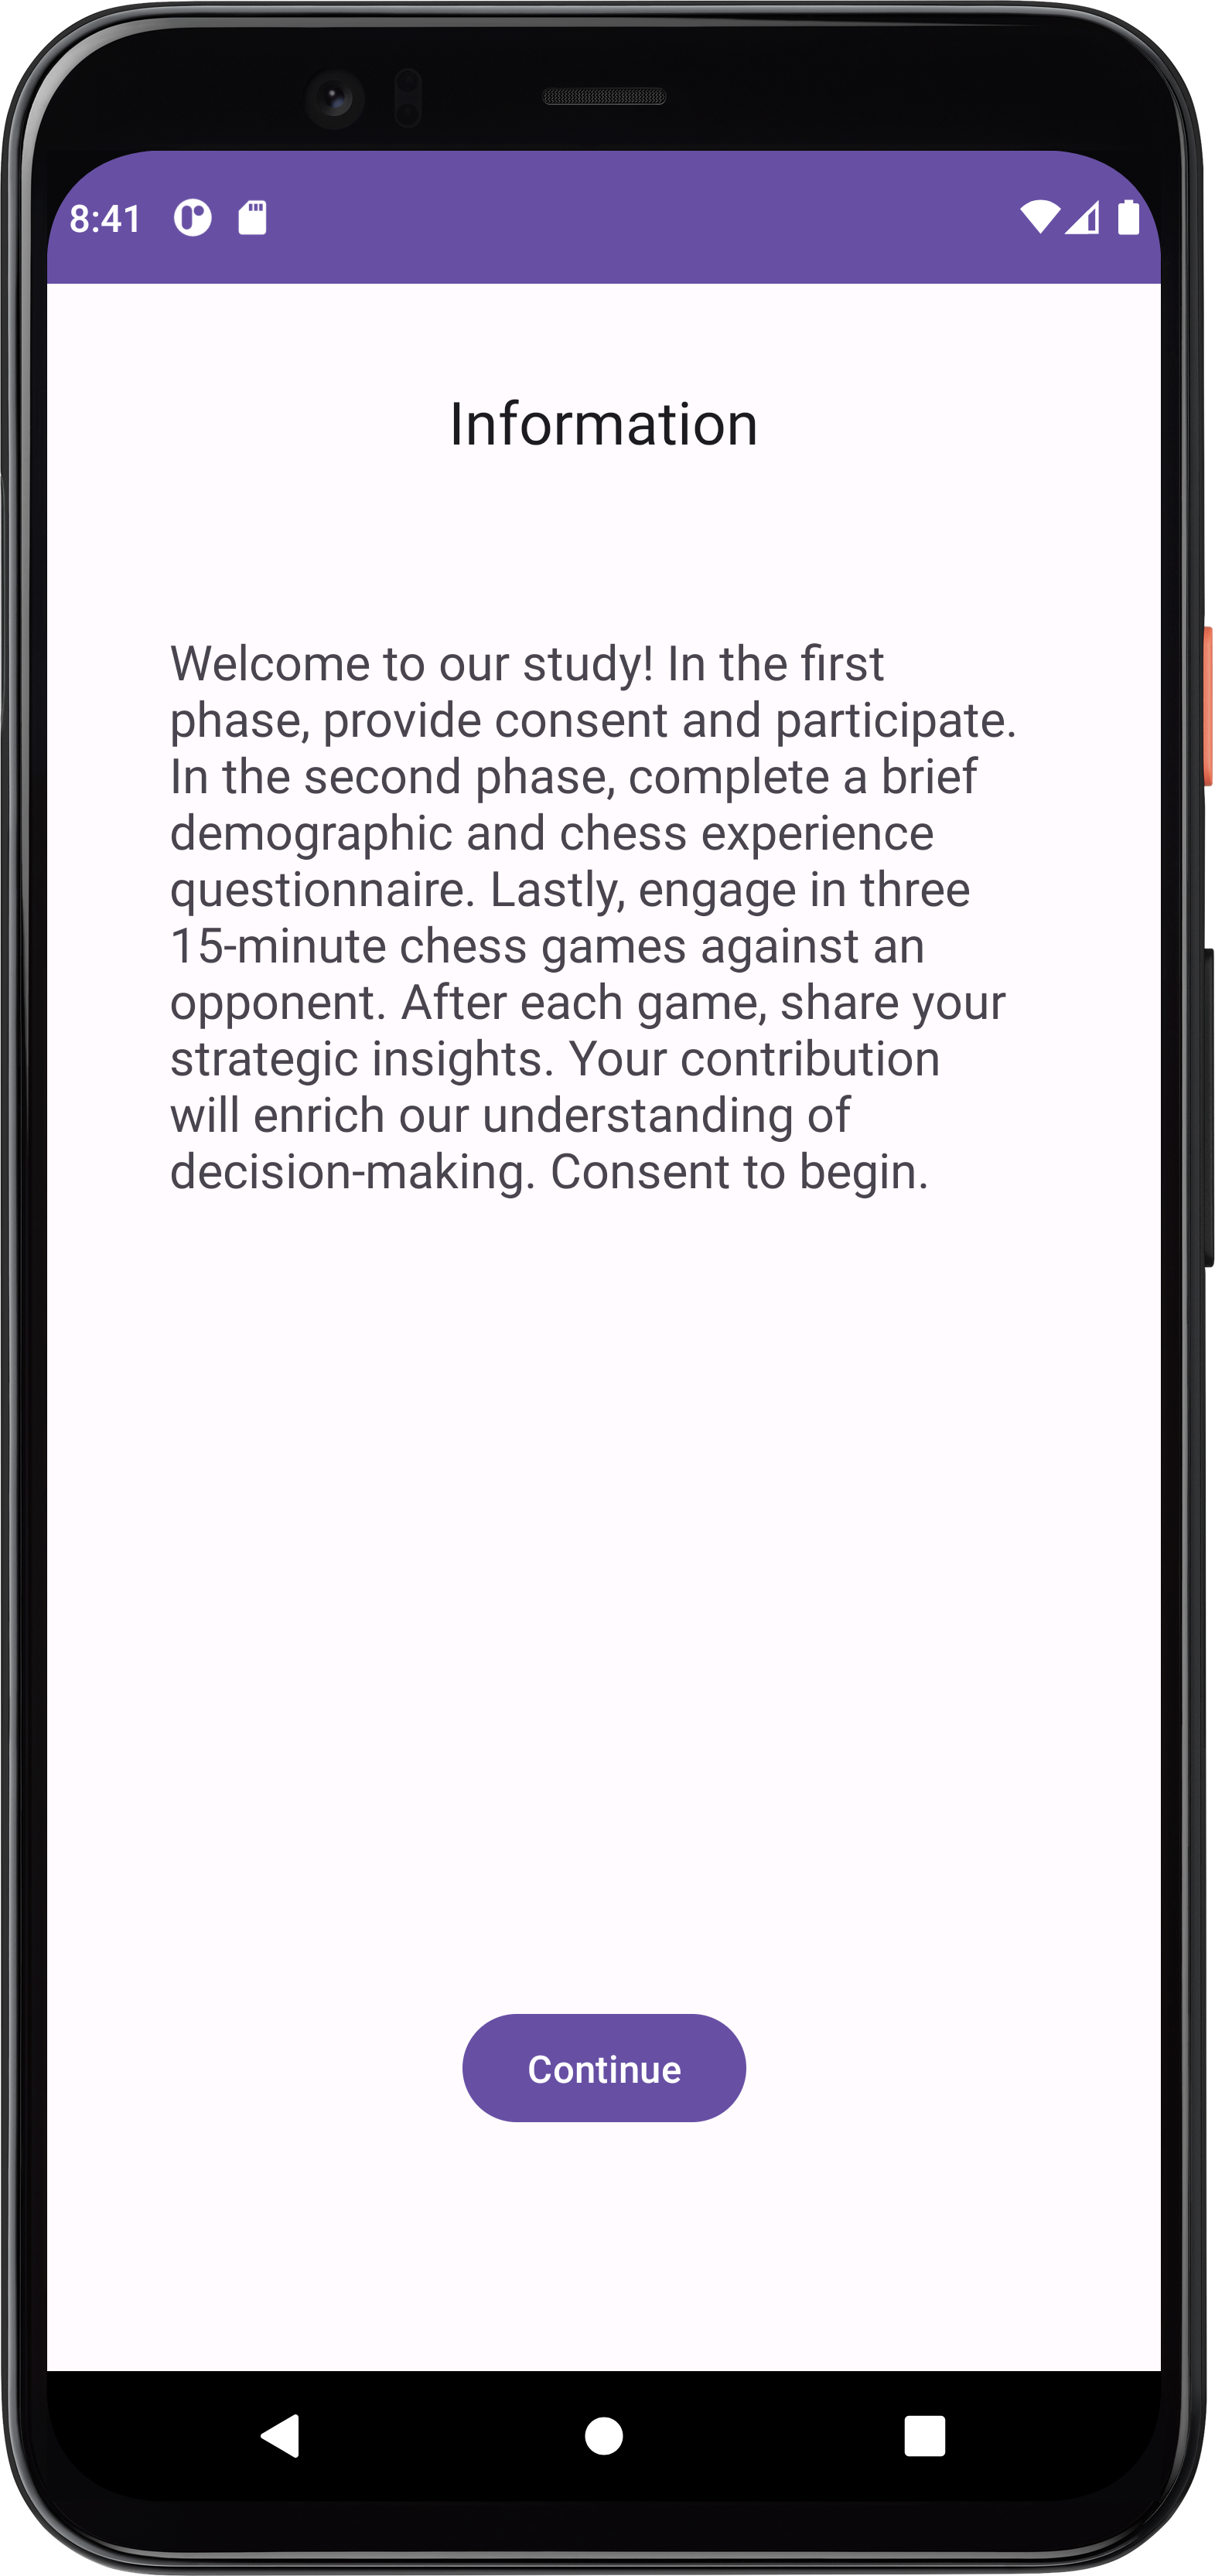
\includegraphics[width=\textwidth]{content/06_demonstration_of_the_artifact/Screenshot_InfoScreen.png}
        \caption{Choose subject step}
        \label{subfig:chooseTestSubject2}
    \end{subfigure}
    %\hfill
    \hspace{1cm}
    \begin{subfigure}[b]{0.25\textwidth}
        \centering
        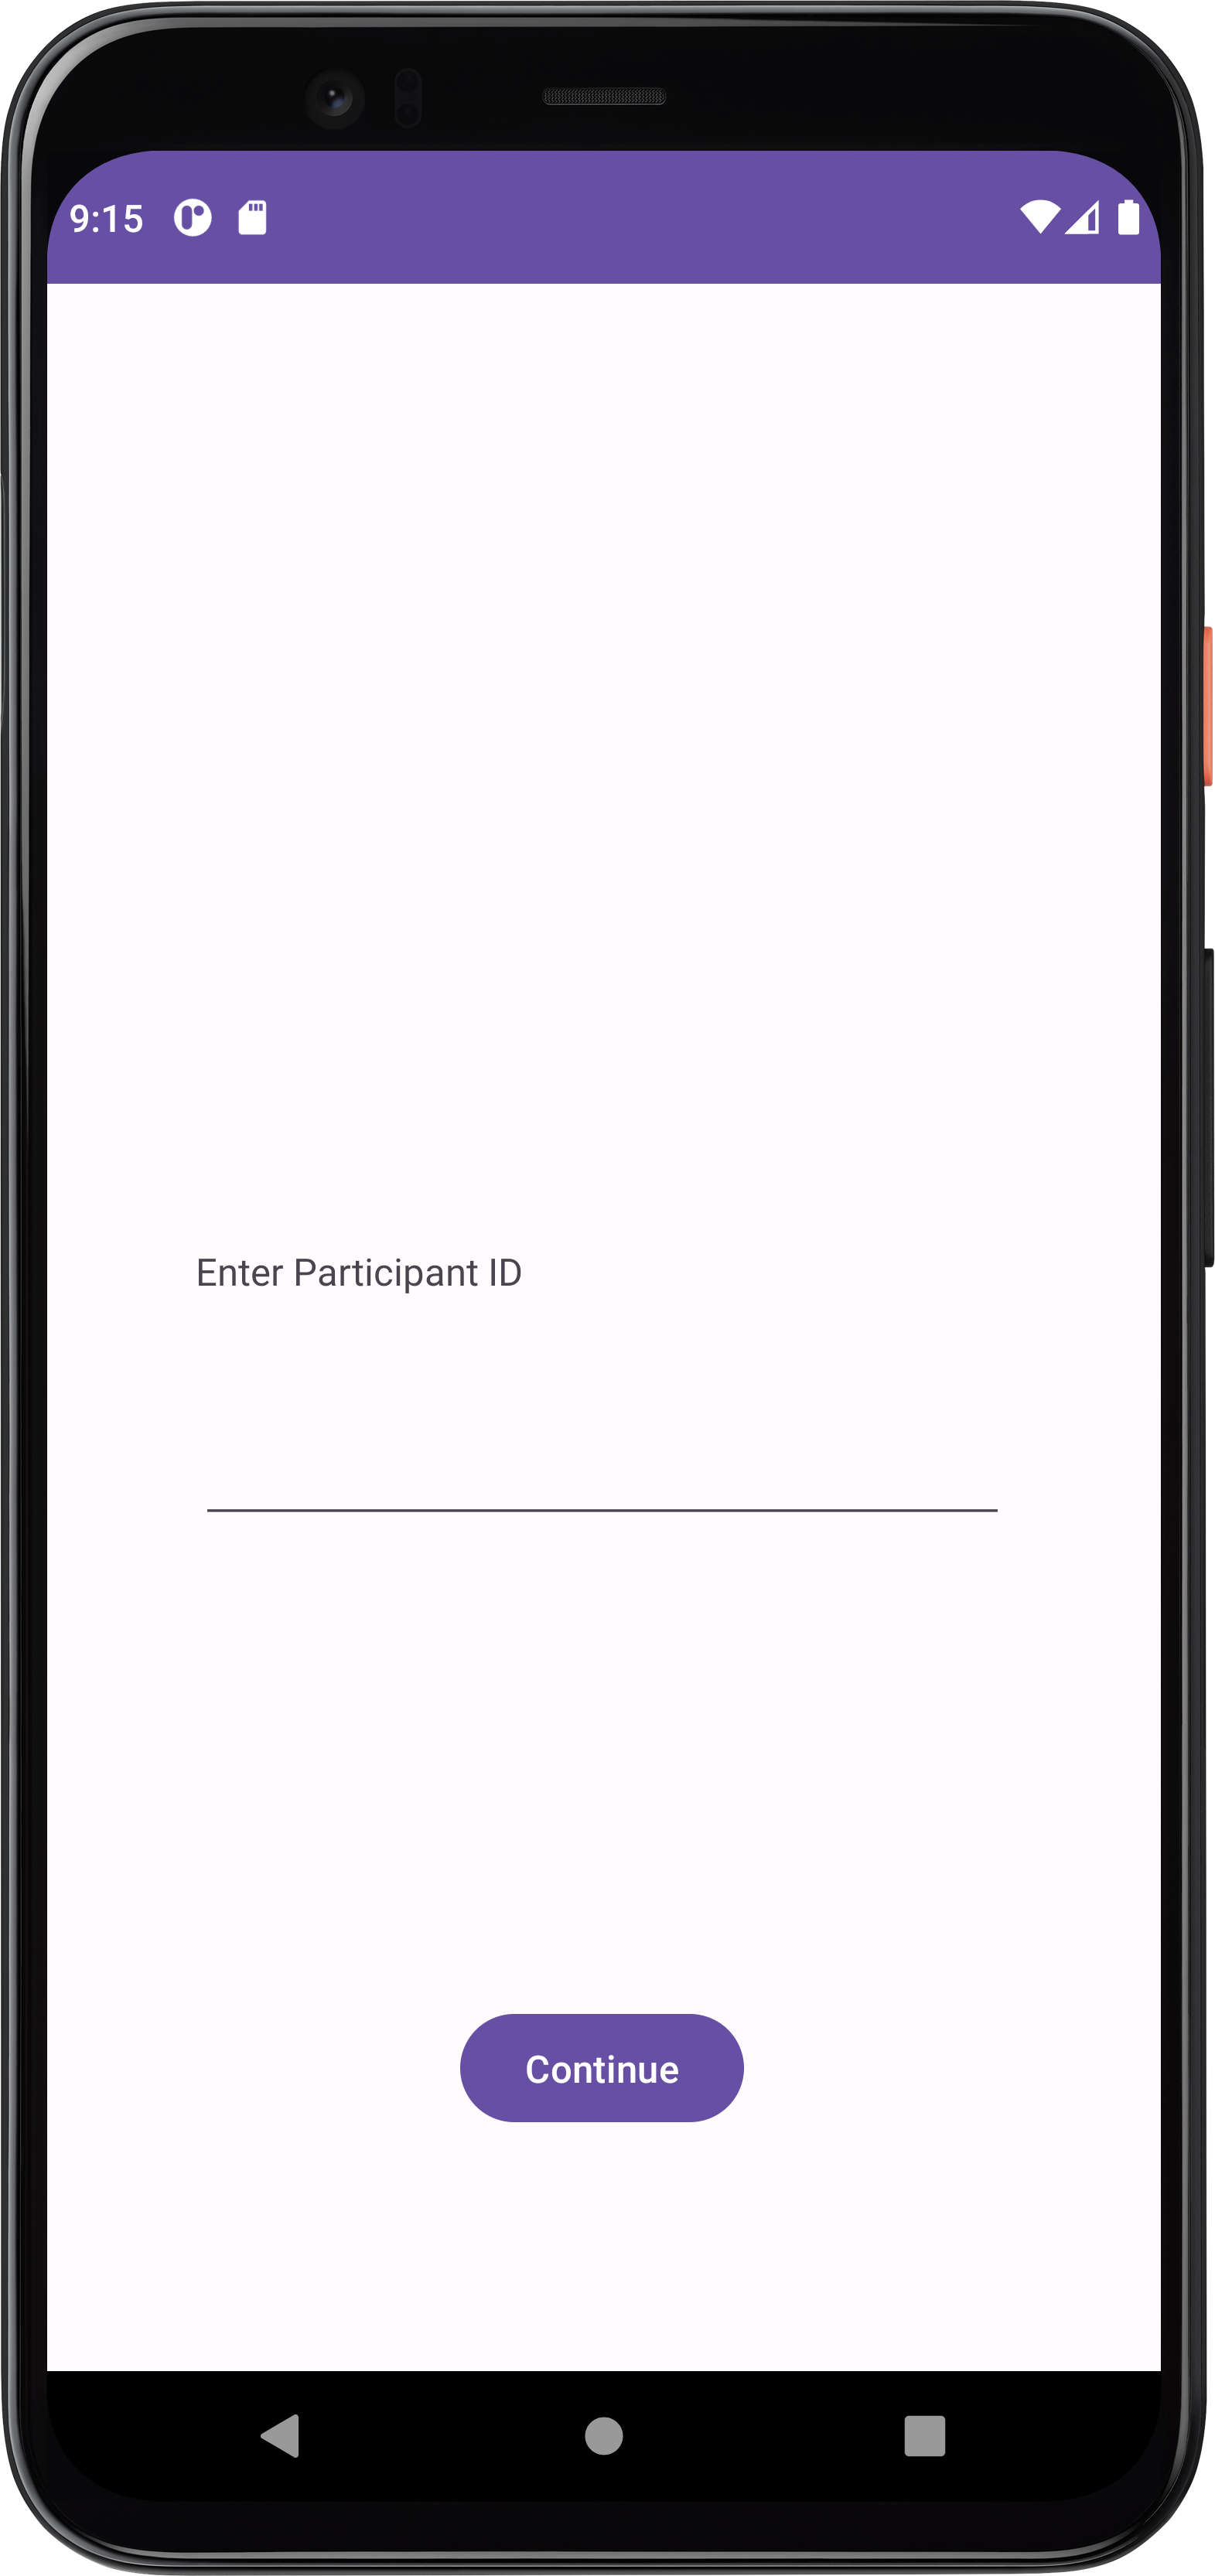
\includegraphics[width=\textwidth]{content/06_demonstration_of_the_artifact/Screenshot_ParticipantSelectionScreen.png}
        \caption{Questionair step}
        \label{subfig:Questionair2}
    \end{subfigure}
        %\hfill
    \hspace{1cm}
    \begin{subfigure}[b]{0.25\textwidth}
        \centering
        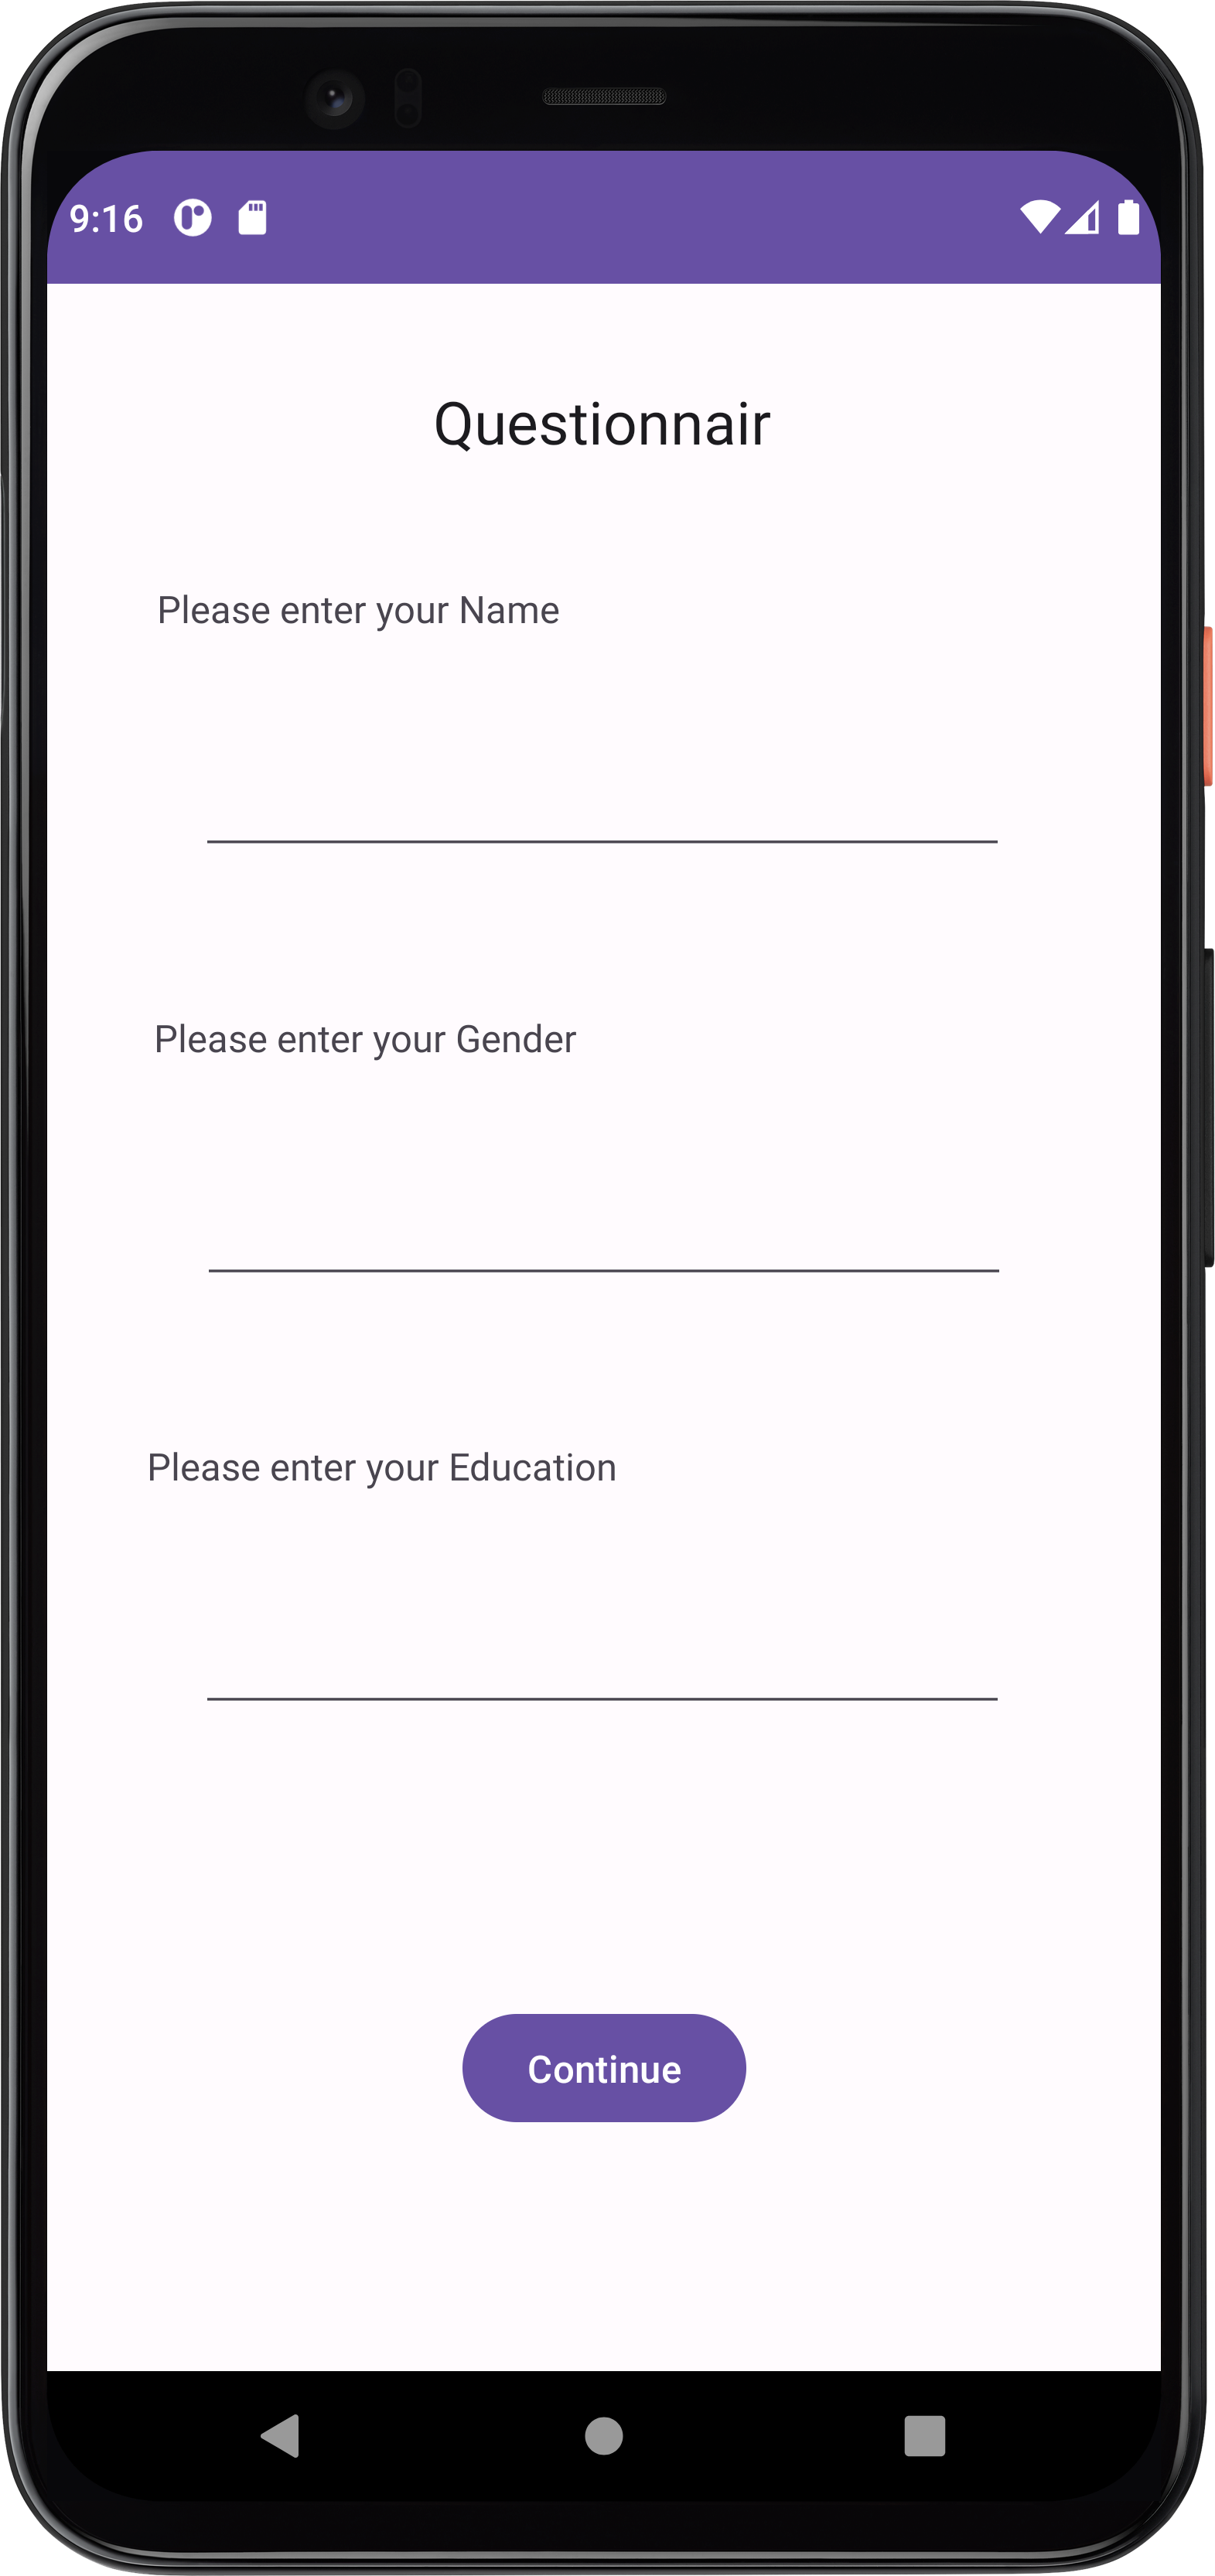
\includegraphics[width=\textwidth]{content/06_demonstration_of_the_artifact/Screenshot_QuestionnairScreen.png}
        \caption{Info screen step}
        \label{subfig:InfoScreen2}
    \end{subfigure}
       \caption{User Interface Prototype of Artefact}
       \label{fig:uiScreens}
\end{figure}

For changing or adding the individual steps of the application, only the sequence data of the experiment must be changed. The same applies to the Information Screen or the Questionnair step. New experiments can build on the existing UseCases in the domain layer and extend them in the course of object-oriented programming. If additional experiment steps contain \ac{ui} interactions, these are implemented via new Android Activities. The name of the activity must then only be stored in the experiment data as a string in order to call it. The full program code can be found in the Github repo at: \textit{https:\/\/github.com\/schneemax\/master\_thesis}